\documentclass[12pt,a4paper]{article}
\usepackage[utf8]{inputenc}
\usepackage[T1]{fontenc}
\usepackage{amsmath}
\usepackage{amsfonts}
\usepackage{amssymb}
\usepackage{amsthm}
\usepackage{graphicx}
\usepackage{subfigure}
\usepackage{float}
\newtheorem*{lemma}{Lemma}
\newtheorem*{theorem}{Theorem}
\newtheorem*{corollary}{Corollary}
\newtheorem*{prf}{\textbf{Proof}}
\usepackage{caption}
\DeclareMathOperator{\n}{\nabla}
\DeclareMathOperator{\E}{\mathrm{E}}
\DeclareMathOperator{\xyz}{\textbf{numpy.random.normal()}}
\title{CS331-HW8-Lukang-Sun}
\begin{document}
	\maketitle
	\paragraph{p1.}
	\begin{proof}
		let $u:=prox_{\gamma R}(x), v:=prox_{\gamma R}(y)$, then by definition we have, $0\in \partial R(u)+\frac{1}{\gamma}(u-x),0\in \partial R(v)+\frac{1}{\gamma}(v-y)$, so $x-u-(y-v)\in \gamma (\partial R(u)-\partial R(v))$, by strong convexity of $R$, we have
		\begin{equation}
			\langle x-u-(y-v),u-v\rangle \geq \gamma\lambda ||u-v||_2^2,
		\end{equation}
	so 
	\begin{equation}
		\begin{aligned}
			||x-y||^2&=||x-u-(y-v)+(u-v)||^2\\
						&\geq ||u-v||^2+2\langle x-u-(y-v), u-v\rangle\\
						&\geq (1+2\gamma \lambda)||u-v||^2.
		\end{aligned}
	\end{equation}
This proves the problem.
	\end{proof}
	\paragraph{p2.}
	\begin{theorem}
		Assume that $f$ is $\mu$-convex and $R$ is $\lambda$-convex, $g^{k}$ is unbiased (Assumption 1) and that the AC assumption (Assumption 2) is satisfied. Choose a stepsize satisfying
		$$
		0<\gamma \leq \frac{1}{A}
		$$
		Then the iterates $\left\{x^{k}\right\}_{k \geq 0}$ of SGD (Algorithm 3) satisfy
		$$
		E\left[\left\|x^{k}-x^{\star}\right\|^{2}\right] \leq(\frac{1-\mu\gamma}{1+2\lambda\gamma})^k||x^0-x^{\star}||^2+ \frac{C\gamma}{\mu(1+2\lambda\gamma)}
		$$
	\end{theorem}
	\begin{proof}
		 let $r^{k} \stackrel{\text { def }}{=} x^{k}-x^{\star} .$ Performing the exact same steps as in the case of GD, but replacing the gradient $\nabla f\left(x^{k}\right)$ by the stochastic gradient $g^{k}$, we get
		$$
		\begin{aligned}
			\left\|r^{k+1}\right\|^{2} & =\left\|\operatorname{prox}_{\gamma R}\left(x^{k}-\gamma g^{k}\right)-x^{\star}\right\|^{2} \\
			& \stackrel{}{=}\left\|\operatorname{prox}_{\gamma R}\left(x^{k}-\gamma g^{k}\right)-\operatorname{prox}_{\gamma R}\left(x^{\star}-\gamma \nabla f\left(x^{\star}\right)\right)\right\|^{2} \\
			& \stackrel{(p1.)}{\leq}\frac{1}{1+2\gamma\lambda}\left\|\left(x^{k}-\gamma g^{k}\right)-\left(x^{\star}-\gamma \nabla f\left(x^{\star}\right)\right)\right\|^{2} \\
		    & =\frac{1}{1+2\gamma\lambda}(\left\|x^{k}-x^{\star}-\gamma\left(g^{k}-\nabla f\left(x^{\star}\right)\right)\right\|^{2}) \\
			& =\frac{1}{1+2\gamma\lambda}(\left\|r^{k}\right\|^{2}-2 \gamma\left\langle r^{k}, g^{k}-\nabla f\left(x^{\star}\right)\right\rangle+\gamma^{2}\left\|g^{k}-\nabla f\left(x^{\star}\right)\right\|^{2}),
		\end{aligned}
		$$
		so 
		$$
		\begin{aligned}
			\mathrm{E}\left[\left\|r^{k+1}\right\|^{2} \mid x^{k}\right] & \leq\frac{1}{1+2\gamma\lambda}(\left\|r^{k}\right\|^{2}-2 \gamma \mathrm{E}\left[\left\langle r^{k}, g^{k}-\nabla f\left(x^{\star}\right)\right\rangle \mid x^{k}\right]+\gamma^{2} \mathrm{E}\left[\left\|g^{k}-\nabla f\left(x^{\star}\right)\right\|^{2} \mid x^{k}\right]) \\
			&=\frac{1}{1+2\gamma\lambda}(\left\|r^{k}\right\|^{2}-2 \gamma\left\langle r^{k}, E\left[g^{k} \mid x^{k}\right]-\nabla f\left(x^{\star}\right)\right\rangle+\gamma^{2} E\left[\left\|g^{k}-\nabla f\left(x^{\star}\right)\right\|^{2} \mid x^{k}\right]) \\
			& \stackrel{}{=}\frac{1}{1+2\gamma\lambda}(\left\|r^{k}\right\|^{2}-2 \gamma\left\langle r^{k}, \nabla f\left(x^{k}\right)-\nabla f\left(x^{\star}\right)\right\rangle+\gamma^{2} E\left[\left\|g^{k}-\nabla f\left(x^{\star}\right)\right\|^{2} \mid x^{k}\right]),
		\end{aligned}
		$$
		use $$
		\left\langle r^{k}, \nabla f\left(x^{k}\right)-\nabla f\left(x^{\star}\right)\right\rangle \stackrel{}{\geq} D_{f}\left(x^{k}, x^{\star}\right)+\frac{\mu}{2}\left\|x^{k}-x^{\star}\right\|^{2},
		$$
		lead to 
		$$
		E\left[\left\|r^{k+1}\right\|^{2} \mid x^{k}\right] \leq\frac{1}{1+2\gamma\lambda}\left((1-\gamma \mu)\left\|r^{k}\right\|^{2}-2 \gamma D_{f}\left(x^{k}, x^{\star}\right)+\gamma^{2} E\left[\left\|g^{k}-\nabla f\left(x^{\star}\right)\right\|^{2} \mid x^{k}\right]\right),
		$$
		use Assumption (2), we get 
		$$
			E\left[\left\|r^{k+1}\right\|^{2} \mid x^{k}\right] \leq \frac{1}{1+2\lambda\gamma}(1-\gamma\mu)||r^k||^2+\frac{1}{1+2\lambda\gamma}{\gamma^2C},
		$$
		so we have 
		$$
		E\left[(1+2\lambda\gamma)^k||r^k||^2\right]\leq (1-\mu\gamma)^k||r^0||^2+\frac{\gamma C(1+2\lambda\gamma)^{k-1}}{\mu},
		$$
		divide by $(1+2\lambda\gamma)^k$ from both sides, we have 
		$$
		E\left[||r^k||\right]\leq (\frac{1-\mu\gamma}{1+2\lambda\gamma})^k||r^0||^2+ \frac{C\gamma}{\mu(1+2\lambda\gamma)}
		$$
	\end{proof}

	\paragraph{p3.}
	(i)
	\begin{equation*}
		E\left[g^k\mid \mathcal{F}_k(y)\right]=(1-q)\nabla f(y^k)+q(\frac{1}{q}\nabla f(x^k)+(1-\frac{1}{q})\nabla f(y^k))=\nabla f(x^k)
	\end{equation*}
	(ii)
	\begin{lemma}
		Assume $f$ is $\mu$-convex and $L$-smooth, $R$ is convex, then we have 
		$$
		\mathrm{E}\left[\left\|g^{k}-\nabla f\left(x^{\star}\right)\right\|^{2} \mid x^{k}, \xi^{k}\right] \leq 2 A D_{f}\left(x^{k}, x^{\star}\right)+B \sigma^{k},
		$$
		$$
		\mathrm{E}\left[\sigma^{k+1} \mid x^{k}, \xi^{k}\right] \leq 2 \tilde{A} D_{f}\left(x^{k}, x^{\star}\right)+\tilde{B} \sigma^{k},
		$$
		where $\sigma^k=\E\left[||\nabla f(y^k)-\nabla f(x^{\star}) ||^2\right]$, $A=\frac{2L}{q},B=1-q+\frac{2(1-q)^2}{q},\tilde{A}=pL,\tilde{B}=(1-p)$.
	\end{lemma}
	\begin{theorem}
		Assume that $f$ is $\mu$-convex.For any $M>\frac{B}{1-\tilde{B}}$ choose a stepsize $\gamma$ satisfying
		$$
		0<\gamma \leq \min \left\{\frac{1}{\mu}, \frac{1}{A+M \tilde{A}}\right\}
		$$
		Then the iterates $\left\{x^{k}, \sigma^{k}\right\}_{k \geq 0}$ of SGD-CTRL satisfy
		$$
		\mathrm{E}\left[V^{k}\right] \leq \max \left\{(1-\gamma \mu)^{k},\left(\frac{B+M \tilde{B}}{M}\right)^{k}\right\} V^{0}
		$$
		where the Lyapunov function $V^{k}$ is defined by
		$$
		V^{k} \stackrel{\text { def }}{=}\left\|x^{k}-x^{\star}\right\|^{2}+M \gamma^{2} \sigma^{k}
		$$
	\end{theorem}
	\begin{proof}
		We only need to prove the lemma, the theorem is a corollary of the lemma.
		\begin{equation*}
			\begin{aligned}
				&\E\left[||g^k-\nabla f(x^{\star})||^2\mid k\right]=(1-q)||\nabla f(x^k)-\nabla f(x^{\star})||^2\\
				&+q||1/q (\nabla f(x^k)-\nabla f(x^{\star}))+(1-1/q)(\nabla f(y^k)-\nabla f(x^{\star}))||^2\\
				&\leq (1-q+\frac{2(1-q)^2}{q})||\nabla f(y^k)-\nabla f(x^{\star})||^2+2(\frac{2L}{q})D_f(x^k,x^{\star})
			\end{aligned}
		\end{equation*}
		\begin{equation*}
			\begin{aligned}
				\E\left[||\nabla f(y^{k+1})-\nabla f(x^{\star})||^2\mid k\right]&=(1-p)||\nabla f(y^k)-\nabla f(x^{\star})||+p||\nabla f(x^k)-\nabla f(x^{\star})||^2\\
				&\leq(1-p)\sigma^k+2(pL)D_f(x^k,x^{\star}).
			\end{aligned}
		\end{equation*}
		\end{proof}
	(iii)when $p\approx 1,q\approx 1$, this method perform well, when $p\approx 0,q\approx 0$, this method performs poorly. This method will reduce the computation of the gradient, so when it is very expensive to compute the gradient(like the dimension is very large), then this method might be a good substitute of gradient descent method.
	In my experiment,  $f=x^2+0.5y^2$,step size $\gamma = 0.005$, I get the results in terms of different $p,q$. 
	
	\begin{figure}
		\centering
		\subfigure[ ]{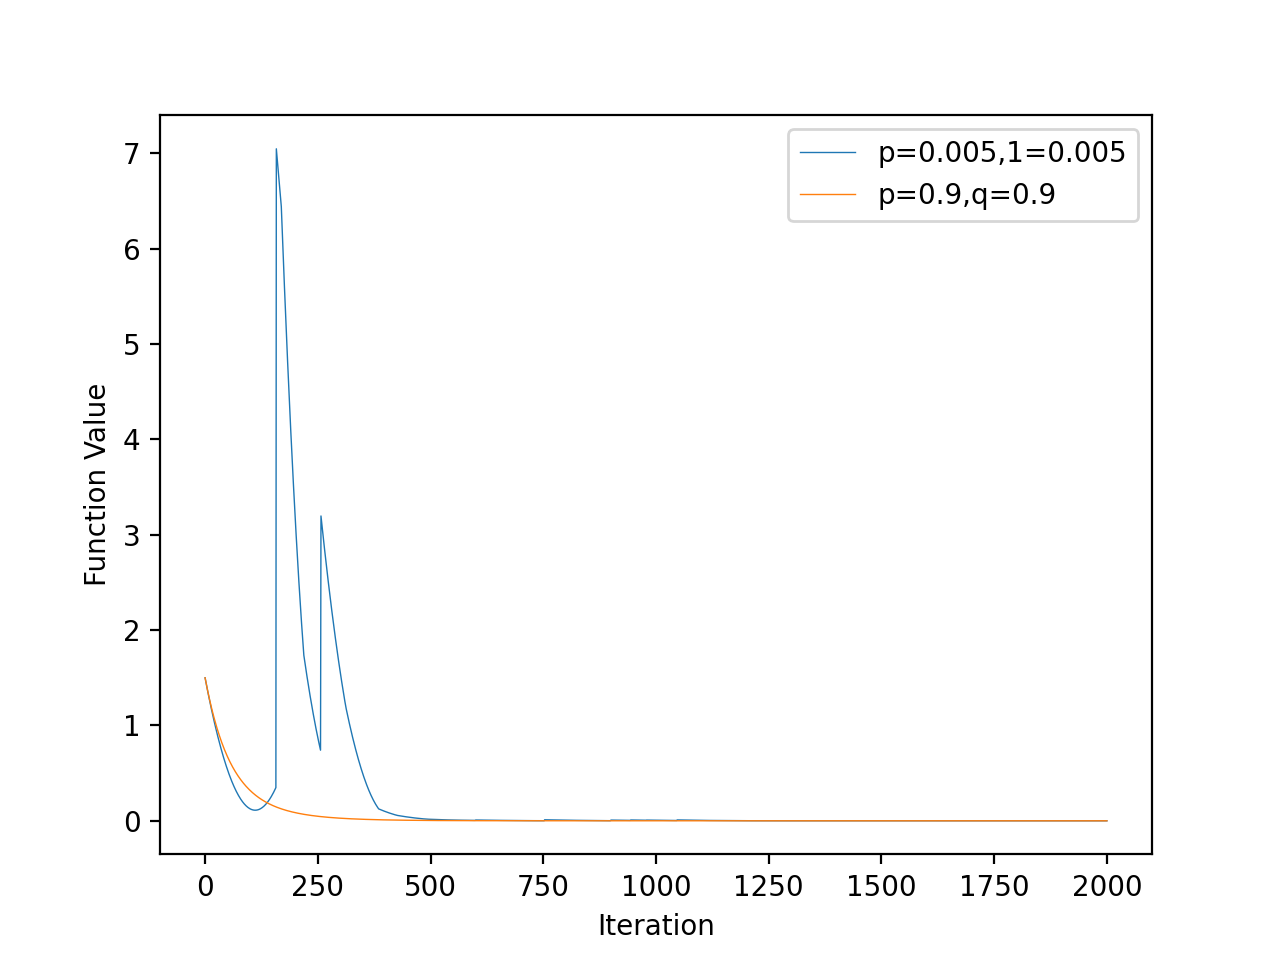
\includegraphics[width=6.7cm]{Figure_81.png}} 
		\subfigure[]{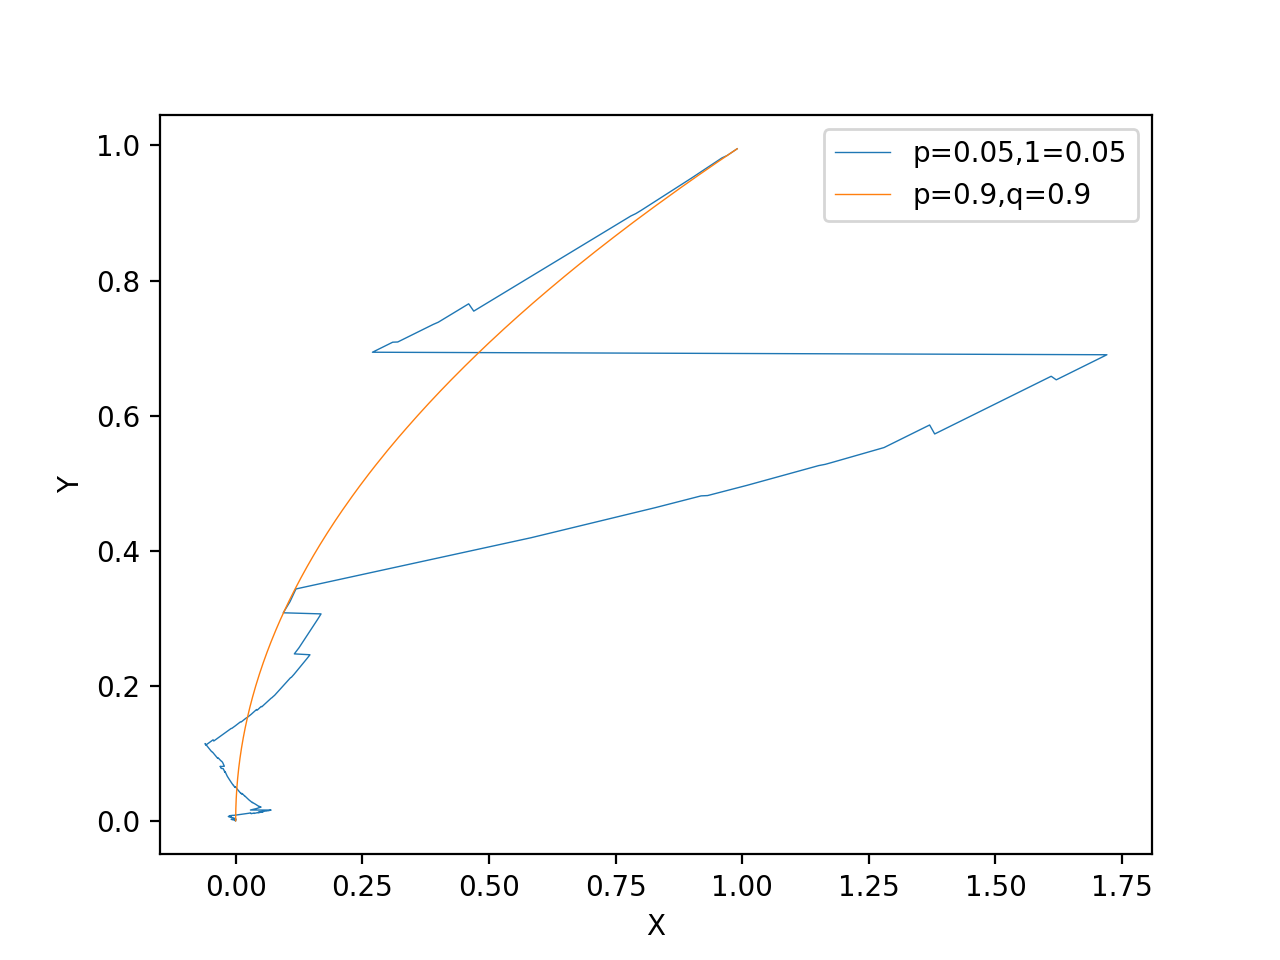
\includegraphics[width=6.7cm]{Figure_82.png}}
		
		
		\caption{ (a) shows function value change in terms of iteration,(b)  shows the trajectories of this method with different $p,q$.you can see that when $p,q$ are close to 1,  this method converges quite smoothly, when $p,q$ are close to 0, this method converges with fluctuations, this match the theory.} %图片标题
		\label{img2}
	\end{figure}
	
	
	
	
	
	
	
	
	
	
	
	
	
	
	
	
	
	
	
	
	
	
	
	
	
	
	
	
	
\end{document}